\documentclass[12pt]{article}

\usepackage{sbc-template}

\usepackage{graphicx,url}

\usepackage{amsmath}

\usepackage{mathtools}

\usepackage[section]{placeins}

\usepackage[brazil]{babel}   

\usepackage[utf8]{inputenc} 

\usepackage{xcolor}

\usepackage{listings}

\newcommand\tab[1][1cm]{\hspace*{#1}}

\definecolor{mGreen}{rgb}{0,0.6,0}
\definecolor{mGray}{rgb}{0.5,0.5,0.5}
\definecolor{mPurple}{rgb}{0.58,0,0.82}
\definecolor{backgroundColour}{rgb}{0.95,0.95,0.92}

\lstdefinestyle{CStyle}{
    backgroundcolor=\color{backgroundColour},   
    commentstyle=\color{mGreen},
    keywordstyle=\color{magenta},
    numberstyle=\tiny\color{mGray},
    stringstyle=\color{mPurple},
    basicstyle=\footnotesize,
    breakatwhitespace=false,         
    breaklines=true,                 
    captionpos=b,                    
    keepspaces=true,                 
    numbers=left,                    
    numbersep=5pt,                  
    showspaces=false,                
    showstringspaces=false,
    showtabs=false,                  
    tabsize=2,
    language=C
}

     
\sloppy

\title{Análise de Paralelismo\\ Cholesky}

\author{Paulo Alexandre Piornedo Panucci\inst{1}}


\address{Departamento de Informática -- Universidade Estadual de Maringá
  (UEM)\\
  \email{ra88380@uem.br}
}

\begin{document} 

\maketitle

\begin{abstract}
A sequential code can be written to be parallel executed in a set of threads, with the purpose of taking advantage of the core quantity in a machine, making the program execution faster. It is expected that making a program parallel, it has a significantly better execution time than the sequential program, although there are cases in which the parallelized code has a similar or worst performance compared to the sequential code. In this work will be analyzed the parallel version of Cholesky's algorithm to matrix decomposition, showing that this parallel version does not reach a good performance concerning its sequential version. 
\end{abstract}
     
\begin{resumo}
Um código sequencial pode ser escrito para ser executado paralelamente em um conjunto de \textit{threads}, com finalidade de tirar proveito da quantidade de núcleos presentes em uma máquina e assim tornar a execução do programa mais rápida. Espera-se que ao paralelizar um determinado programa, ele possua um tempo significantemente melhor que o código sequencial, mas também existem casos em que um código paralelizado tem um desempenho próximo, ou pior, que o sequencial. Neste trabalho será analisada a paralelização do algoritmo Cholesky para decomposição de matrizes, mostrando que este algoritmo não alcança um bom desempenho paralelizando-o com referência no código sequencial.  
\end{resumo}


\section{Introdução}\label{sec:intro}

\tab Como observado por \cite{aubanel:1606499}, antes da revolução dos processadores \textit{multicore}, o programador dependia das melhoras de performance apresentadas por processadores conforme o lançamento de novas gerações. Com a estagnação do aumento da taxa de \textit{clock}, poder utilizar múltiplos \textit{cores}  para conseguir rodar um programa tende a tornar a execução mais eficiente dependendo como este problema é modelado.
\\
\tab Hoje conta-se com diretivas de compilação e APIs para paralelizar um código. Um exemplo é o \textit{OpenMP} para a linguagem C/C++. Apesar de existirem alternativas de deixar o trabalho de paralelização para o compilador, aprender a escrever códigos paralelos distribuídos tem suas vantagens. \cite{aubanel:1606499} ainda diz que os compiladores tentam otimizar o código que é dado a eles, porém eles não reescrevem esse código para que ele realmente seja paralelo. Desta forma pode-se dizer que existe uma diferença entre paralelizar um código em C com o OpenMP e escrever um código paralelo utilizando a biblioteca Pthread do C.

\section{Fundamentação Teórica} \label{sec:fund}

\tab Este trabalho abordará a análise de paralelismo do algoritmo da decomposição de Cholesky. Desta forma, é importante se conhecer o objetivo desta decomposição, assim como alguns conceitos básicos de paralelismo para se entender esta análise. 

\subsection{Decomposição de Cholesky}\label{subsec:chol}
\tab A decomposição de Cholesky consiste em: dada uma matriz A simétrica e positiva definida, existe uma matriz triangular inferior L tal que multiplicada por sua transposta o resultado seja A. Logo, esta decomposição pode ser definida pela seguinte fórmula: 
\begin{center}
$A = \text{L} \times \text{L}^\text{T}$.
\end{center}
\tab Uma matriz simétrica consiste em uma matriz no qual sua transposta é igual a ela mesma. Ou seja: 
\begin{center}
$A = \text{A}^\text{T}$.
\end{center}
\tab Uma matriz é definida positiva caso todos os seus auto-valores são maiores que zero. 

\subsection{Paralelismo}\label{subsec:paralel}

\tab Serão abordados agora alguns conceitos básicos importantes para se entender o paralelismo a nível de thread e sua análise.

\subsubsection{\textit{Speedup}}\label{subsubsec:speedup}
\tab Ao se escrever um código paralelo a partir de um sequencial, espera-se que seu código paralelo tenha um desempenho de tempo que se aproxima de N vezes melhor que o tempo do código sequencial, sendo este N o número de threads que serão executadas em paralelo, e este valor é dado pelo \textit{speedup}. 
\\
\tab Quando dividimos o tempo de execução do algoritmo sequencial pelo tempo de execução do algoritmo paralelo, tem-se então o seu \textit{speedup}: 
\begin{center}
$S_p = \frac{T_s}{T_p}$. 
\end{center}
\tab É importante distinguir o tempo decorrido da execução do código, do tempo total levado pela soma dos tempos de execução de cada \textit{thread}. Para fim de análise de speedup precisa-se do \textit{elapsed time}, que é o tempo decorrido do começo ao fim do programa (ou de uma função paralela específica). 
\\
\tab Quando o \textit{speedup} de um determinado programa paralelo possui um valor maior que o número de \textit{threads} que executa este código, tem-se então um \textit{speedup} dito superescalar.

\subsubsection{Condição de Corrida}\label{subsubsec:racecond}
\tab Ao se escrever um código paralelo, quando \textit{threads} simultâneas podem competir por algum recurso diz-se que existe condição de corrida neste algoritmo. Pode-se definir como recursos acesso em uma determinada região da memória, e até mesmo o próprio hardware em que o algoritmo está sendo executado. Como um exemplo de disputa de recursos, pode se dar o exemplo que uma determinada \textit{thread} queira escrever ao mesmo tempo que outra em uma região da memória, ou também a primeira quer ler um resultado que está ao mesmo tempo sendo escrita pela segunda. Como exemplo de disputa de recurso de \textit{hardware}, uma quantidade x de \textit{threads} que estão prontas para ser executadas, porém a máquina contém $\frac{x}{2}$ núcleos de processamento.
\\
\tab Para se resolver problemas de condição de corrida, principalmente de software, deve se usar recursos como \textit{locks} e barreiras. 
\\
\tab Se existe alguma região crítica em que somente uma \textit{thread} pode estar executando essa região, pode-se utilizar \textit{lock} para não deixar que outras \textit{threads} acessem essa área e \textit{unlock} para liberar para as outras.
\\
\tab Ao se procurar por sincronia em um algoritmo, opta-se pelo uso de barreiras. Quando uma barreira é colocada no algoritmo, isso implica que todas as \textit{threads} devem chegar na mesma região para assim poder dar continuidade na execução.
\\
\tab Ter condições de corrida no algoritmo que deseja paralelizar implica em diminuir a possibilidade de ter um \textit{speedup} próximo a quantidade de \textit{threads} que estão executando. Isto se dá pelo fato de impedir que as \textit{threads} dependam delas mesmas para executar o trabalho que a ela foi dado.

\subsubsection{Balanceamento de Carga}\label{subsubsec:cargabalanc}
\tab Independente de como é feita a implementação de um código paralelo, é interessante que \textit{threads} tenham um balanceamento execução, ou seja, façam quantidades de trabalho parecidas, para assim alcançar uma melhor performance. 
\\
\tab Em Pthread consegue-se enxergar nitidamente o balanceamento ou a falta dele, pelo fato de isso ter que ser explicitado pelo programador. 

\subsection{Ferramentas}\label{subsec:cargabalanc}
\tab Serão apresentadas algumas ferramentas utilizadas para  o desenvolvimento do  algoritmo paralelo e sua análise.
\subsubsection{Polybench}
\tab O Polybench é uma coleção de \textit{benchmarks} contendo partes de controle estático, com o propósito de uniformizar a execução e o monitoramento de kernels. 
\\
\tab Desta coleção de \textit{benchmarks} que se teve como base de analise o algoritmo de Cholesky.  

\subsubsection{OpenMP}\label{subsubsec:omp}
\tab A ferramenta \textit{OpenMP} é uma \textit{API} que dá suporte a programação paralela em memória compartilhada para C/C++ e Fortran.
\\
\tab Esta ferramenta funciona declarando a diretiva "\#pragma omp parallel" seguida de alguns argumentos nos locais em que deseja paralelizar o código. Fica à cargo do compilador decidir como esse código será então paralelizado. 
\subsubsection{Pthread}\label{subsubsec:pthread}
\tab Pthread é uma biblioteca para a linguagem C em sistemas \textit{UNIX} que como especificado por \cite{pthread} padroniza a programação em threads nesse ambiente.
\\
\tab Ao se tratar de uma biblioteca de criação de threads, fica a cargo do programador em ditar a maneira como a paralelização funcionará. Desta forma deve-se criar threads e passar uma função como argumento para ser executada. Deve-se também fazer a junção dessas threads  e se precisar, matá-las.
\subsubsection{PAPI}\label{subsubsec:papi}
\tab PAPI se refere á \textit{Performance API project} que segundo \cite{papi} especifica uma \textit{API} padrão para acessar contadores de performance de hardware disponíveis na maioria dos processadores modernos.
\\
\tab Os processadores em que essa \textit{API} é suportada possui um número x de contadores que podem ser usados para coletar dados. O que pode ocorrer é a quantidade de dados diferentes que se quer coletar seja maior que o número de contadores, ou até mesmo alguns dados precisam de mais de um contador, fazendo com que na soma total de dados e contadores necessitados passe a quantidade de contadores disponíveis. Quando isto ocorre a ferramenta faz a multiplexação de dados.  

\subsection{VTune\textsuperscript{\texttrademark}}\label{subsubsec:vtune}
\tab O VTune\textsuperscript{\texttrademark} é um software desenvolvido pela Intel\textsuperscript{\textregistered} para realização de análise de performance em processadores da marca.

\section{Proposta}\label{sec:prop}
\tab Este trabalho tem como proposta desenvolver um algoritmo paralelo da decomposição de matrizes utilizando o método de Cholesky com base num código sequencial presente no Polybench, mostrar que este programa presente no conjunto de \textit{benchmarks} precisa ter uma alteração em sua estrutura sequencial para se tornar paralelo. Através desta alteração, fazer a análise de \textit{speedup} do código paralelo usando Pthread e \textit{OpenMP} em relação ao código sequencial reescrito e ao código original do Polybench, e assim mostrar um baixo desempenho da versão paralela, explicando suas condições de corrida.
\\
\tab Para isto, será apresentado o código do  algoritmo de Cholesky do   Polybench e o código desenvolvido para a proposta de paralelização deste trabalho.
\subsection{Cholesky do Polybench}\label{subsec:polycholesky}
\begin{lstlisting}[style=CStyle]
static void cholesky_polybench(/*PARAMETROS*/){
  int i, j, k;
	#pragma scop
  for (i = 0; i < size; i++) {
     //j<i
     for (j = 0; j < i; j++) {
        for (k = 0; k < j; k++) {
           A[i][j] -= A[i][k] * A[j][k];
        }
        A[i][j] /= A[j][j];
     }
     // i==j case
     for (k = 0; k < i; k++) {
        A[i][i] -= A[i][k] * A[i][k];
     }
     A[i][i] = SQRT_FUN(A[i][i]);
  }
	#pragma endscop
}
\end{lstlisting}

\subsection{Cholesky Proposto}\label{subsec:cholprop}
\begin{lstlisting}[style=CStyle]
static void cholesky_proposto(){
    int i, j, k;
    for(k = 0; k < size; k++){
        A[k][k] = sqrtf(A[k][k]);
        for(j = (k + 1); j < size; j++){
            A[k][j] /=  A[k][k];
            A[j][k] = A[k][j];
        }
        for(i = (k + 1); i < size; i++){
            for(j = i; j < size; j++){
                A[i][j] -=  A[k][i] *  A[k][j];
                A[j][i] = A[i][j];
            }
        }
    }
    for(i = 0; i < size; i++){
        for(j = i + 1; j < size; j++){
            A[i][j] = 0.0;
        }
    }
}
\end{lstlisting}
\tab O cholesky escrito pela equipe do Polybench faz o procedimento sobre a mesma matriz de entrada, transformando-á em  uma matriz triangular inferior.  No algoritmo proposto se manteve  o mesmo princípio. As operações de divisão e raiz quadrada presentes no algoritmo não podem ser executadas por \textit{threads} simultâneas, sendo um caso de condição de corrida. Neste caso, somente uma  \textit{thread} pode executar  essas operações, e as outras devem esperar a conclusão desta etapa.
\\
\tab Os dois \textit{for loops} entrelaçados seguintes contém uma operação de subtração. Esta etapa é conhecida como etapa de "eliminação". Esta etapa pode ser paralelizada por não apresentar nenhuma condição de corrida. No caso do OpenMP se coloca a diretiva vista na subseção \ref{subsubsec:omp} seguida de alguns parâmetros acima do \textit{for loop} mais externo. No caso do Pthread se define um inicio e um fim nesse laço mais externo, balanceando esse início e fim proporcionalmente entre as \textit{threads} para de alguma forma tentar realizar um balanceamento de carga. Finalizando esse laços entrelaçados,  todas as \textit{threads} devem  começar juntas a etapa de de zerar o triângulo superior da matriz.
\\
\tab Todos os casos citados de sincronização de \textit{threads} usam barreiras.

\section{Ambiente Experimental}\label{sec:amb}
\tab Os algoritmos analisados são desenvolvidos na Linguagem C. São utilizados o OpenMP e Pthread para fazer a versão paralela do código. O PAPI é utilizado como ferramenta de análise. 
\\
\tab Foram analisados então 4 códigos: o código sequencial do Polybench, um código sequencial desenvolvido para se adaptar ao código paralelo, um código paralelo Pthread.
\\
\tab Para a análise de \textit{speedup}, cada código foi executado 11 vezes, sendo a primeira descartada para fim de alimentar a memória \textit{cache}. Nas dez execuções seguintes, salva-se os tempos de execução a biblioteca \textit{time.h} do C, eliminando o melhor e o pior tempo destas, e assim fazendo a média dos tempos que sobraram.
\\
\tab Os algoritmos foram rodados e as análises para speedup coletadas no servidor Pitomba localizado no Departamento de Informática da Universidade Estadual de Maringá. Este servidor conta com 60 núcleos de processamento, sendo 30 deles físico e 128 \textit{GBs} de memória RAM.
\\
\tab Com a ferramenta PAPI foram coletados os seguintes dados, seguindo o mesmo padrão de coleta da análise de \textit{speedup}, porém coletados somente para 8 \textit{threads}:
\begin{itemize}
\item Quantidade de \textit{cache miss} em L1, L2, e L3;
\item Quantidade de ciclos de \textit{clock};
\item Quantidade de instruções completadas.
\end{itemize}
\tab Esta análise com as informações do PAPI foram coletadas em  uma máquina Intel\textsuperscript{\textregistered} i7 8 núcleos, com 8 \textit{GBs} de RAM, disponibilizando 07 contadores para o uso da ferramenta. Esta coleta foi realizada separadamente da coleta de \textit{speedup} pelo fato de o servidor Pitomba não conter a ferramenta PAPI nem uma outra ferramenta de análise de performance, e também não existir a possibilidade de  instalar alguma ferramenta para este fim.
\\
\tab Através do VTune\textsuperscript{\texttrademark}, na mesma máquina utilizada para os testes com o PAPI, foram coletadas amostras de uma execução do código sequencial desenvolvido, uma do \textit{OpenMP} com 8 threads e uma do Pthread também com 8 \textit{threads}.  Foi analisada então o tempo ocioso do processador.

\section{Resultados}\label{sec:res}

\tab Como apresentado por \cite{ruschel:16} a quantidade de dependência de dados influencia na análise de tempo de seu código paralelo, e o Cholesky apresenta implementações variadas com diferentes dependências de dados.  No Cholesky proposto na subseção \ref{subsec:cholprop} vemos as condições de corrida para o paralelismo. Nas figuras \ref{fig:polybench_speedup} e \ref{fig:developed_speedup} vemos respectivamente a análise de \textit{speedup} comparando os códigos paralelos OpenMP e Pthread com o Cholesky sequencial do Polybench e o sequencial do proposto.

\begin{figure}[ht]
\centering
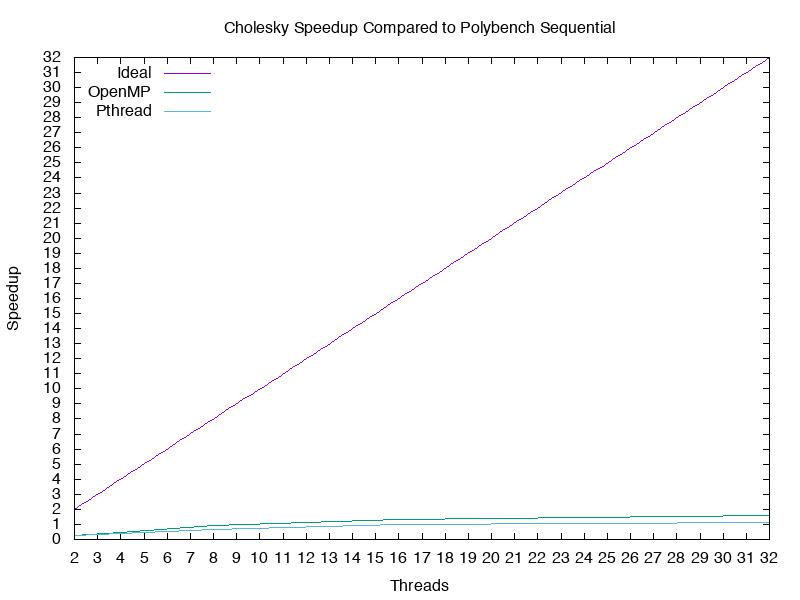
\includegraphics[width=.5\textwidth]{polybench.png}
\caption{Análise de \textit{speedup} a partir do código sequencial do Polybench.}
\label{fig:polybench_speedup}
\end{figure}

\begin{figure}[ht]
\centering
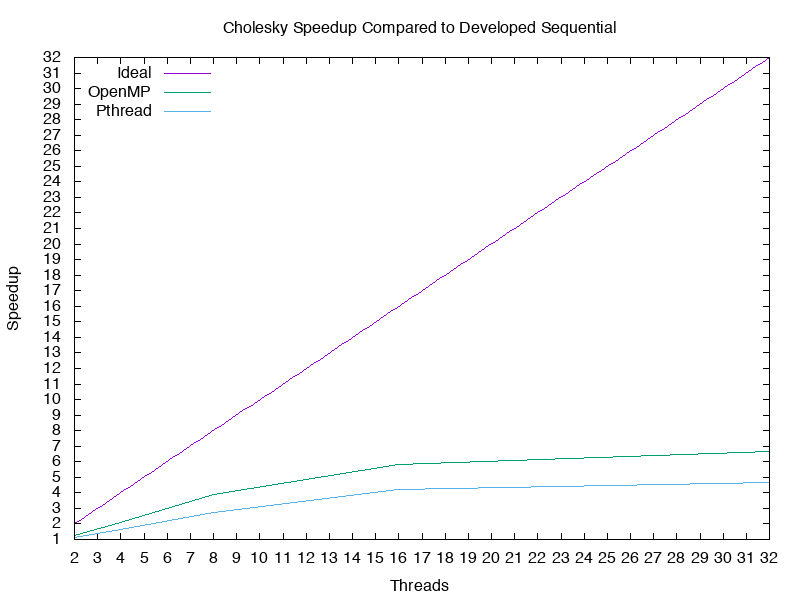
\includegraphics[width=.5\textwidth]{developed.png}
\caption{Análise de \textit{speedup} a partir do código sequencial proposto.}
\label{fig:developed_speedup}
\end{figure}

O desempenho de \textit{speedup} não é bom nem na primeira nem na segunda ocasião, apesar de apresentar melhoras comparando a análise com o mesmo modelo de algoritmo.
\\
\tab Pode-se tentar explicar o mau desempenho de \textit{speedup} analisando 2 informações
\begin{itemize}
\item Quantidade de \textit{cache miss}, caso sendo esta taxa alta motivo de mais acesso a memória principal;
\item{Tempo ocioso do processador}, analisando uma média de instruções por ciclo e o tempo de trabalho do CPU.
\end{itemize}
\tab Como pode ser visto na figura \ref{fig:cache} a taxa de \textit{cache miss} entre o código sequencial e o Pthread é próxima, sendo o segundo  um pouco mais custoso em \textit{misses}. Isso se dá ao fato de a parte em que as \textit{threads} estão trabalhando juntas no código paralelo, elas trabalham em diferentes áreas da matriz, fazendo com que cada \textit{thread} busque informações diferentes das outras, não contendo esse dado na cache, desencadeado mais \textit{cache misses}.
\tab Desta forma, podemos considerar a taxa de \textit{cache miss} um fator que influencia no desempenho geral do algoritmo.

\begin{figure}[ht]
\centering
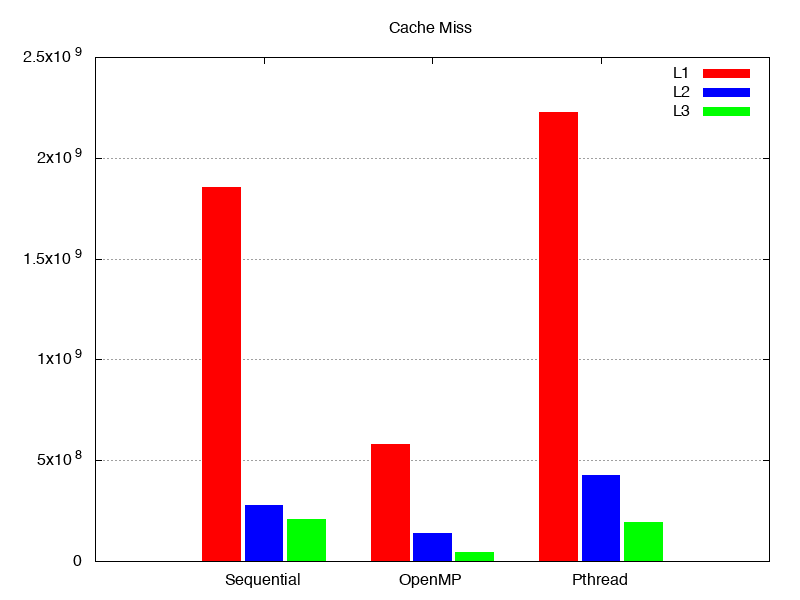
\includegraphics[width=.5\textwidth]{cache.png}
\caption{Análise de \textit{cache miss} 1.}
\label{fig:cache}
\end{figure}

\tab Analisando o uso do processador na figura \ref{fig:cpuinfo} vemos um núcleo com maior parte de trabalho de processamento. Isto se dá pelo fato de ter sido recolhida uma amostragem com um \textit{dataset} menor, e desta forma por este \textit{core} ficar responsável pela inicialização do programa e todas as configurações das matrizes (inicialização e povoamento) ele possui um uso significantemente maior que os outros. Porém pode-se perceber que nem todos os cores apresentam uso balanceado, além de não estar sendo usados todos os 8 presentes na máquina, enquanto numa amostragem do OpenMP está sendo usado. A questão de balanceamento de carga está referida ao motivo explicado na subseção \ref{subsec:cholprop} que somente uma \textit{thread} pode fazer a primeira etapa do algoritmo que é as operações de divisão e raiz quadrada. Enquanto isto é executado, todas as outras \textit{threads} devem esperar para começar a trabalhar. 
\begin{figure}[ht]
\centering
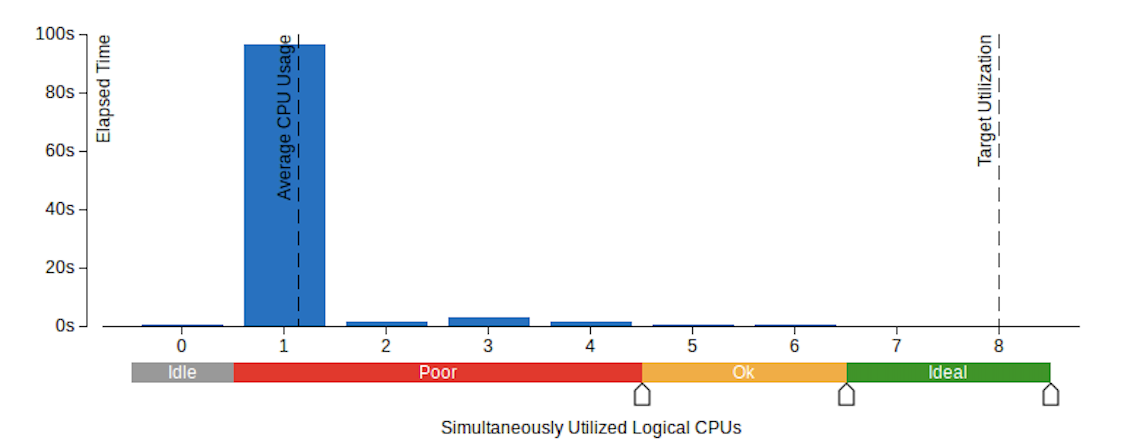
\includegraphics[width=.5\textwidth]{cpu_usage_pthread.png}
\caption{Uso de CPU na execução do Pthread com 8 \textit{threads}}
\label{fig:cpuinfo}
\end{figure}
\\
\tab Esse tempo ocioso da maior parte das \textit{threads} pode ser percebido com os dados coletados pelo PAPI que mostra que para o mesmo \textit{dataset} utilizado na analise de CPU os códigos sequencial  proposto tem uma média de 1,116 instruções por ciclo de \textit{clock}, o OpenMP uma média de 1,26 instruções por ciclo e o Pthread 1,31. O que se espera pensando em um código paralelo a partir do sequencial, é que a relação de instruções por ciclo tenha uma relação crescente proporcional ao número de \textit{threads} que executam no programa. Não se percebe nenhuma mudança significante entre o código sequencial e os paralelos. Isto pode indicar ociosidade de processador, não tendo um balanceamento de carga bom o suficiente para aumentar de alguma maneira a relação de instruções por ciclo.  Uma diferença importante de se lembrar é que o código sequencial acaba sendo executado em um núcleo, enquanto os paralelos deveriam utilizar mais núcleos e assim distribuir o trabalho.
\\
\tab O que pode explicar um melhor desempenho de \textit{speedup} do OpenMP em relação ao Pthread é o tempo ocioso que este último possui e o primeiro não no mesmo nível, devido ao fato de um \textit{for loop} externo do OpenMP ser declarado como paralelizável. Desta forma a primeira parte, que é executada somente por uma \textit{thread} no Pthread fazendo com que as outras fiquem ociosas esperando esta terminar a cada iteração do laço principal, é feita sequencialmente no OpenMP, diminuindo o tempo de ociosidade de outros núcleos.

\section{Conclusão}\label{sec:conc}
\tab Paralelizar o algoritmo sequencial que está contido na coleção de \textit{benchmarks} Polybench exige modificações de forma a permitir lidar com suas condições de corrida. O fato de o algoritmo apresentar uma parte significante de suas operações com condições de corrida faz com que sua paralelização seguindo o modelo do código sequencial apresente um desempenho muito abaixo do esperado em termos de \textit{speedup}. O código paralelo em sua parte paralelizável ao trabalhar em diferentes áreas da matriz de entrada faz com que ocorra bastante \textit{cache miss}, e também a sincronização do algoritmo devido ao grande conflito de dados gerando condições de corrida faz com que o desempenho do \textit{speedup} não seja o tão significante como o esperado. Para uma melhora neste ponto, exige-se uma nova modelagem e abordagem deste algoritmo de decomposição de matrizes.
\\
\tab Apesar do desempenho não tão significante, existe uma melhora de tempo do sequencial para o paralelo. Diminuir o tempo de execução pela metade ou em um quarto pode ser significante quando se pensa em uma escala de tempo maior. Logicamente ter um algoritmo que trabalha mais rápido em cima de um dado problema é vantajoso quando não se tem outras opções. Porém é esperado poder tirar o máximo de vantagem da quantidade de núcleos que se tem disponíveis para processamento, fazendo com que um \textit{speedup} como o apresentado na seção \ref{sec:res} não seja tão interessante.

\bibliographystyle{sbc}
\bibliography{sbc-template}
\end{document}
